\chapter{Tools for Modern Mobile Web Applications}
\label{chapter:tools-and-techniques}

With all the hype and trending surrounding HTML5 and mobile web
applications, several libraries and tools have been developed to help
building these applications. Fling \cite{fling2011anatomy} represents
a typical anatomy of a mobile HTML5 application as shown in
Figure~\ref{figure:anatomy-of-a-html5-mobile-app.png}.

\begin{figure}[h!]
  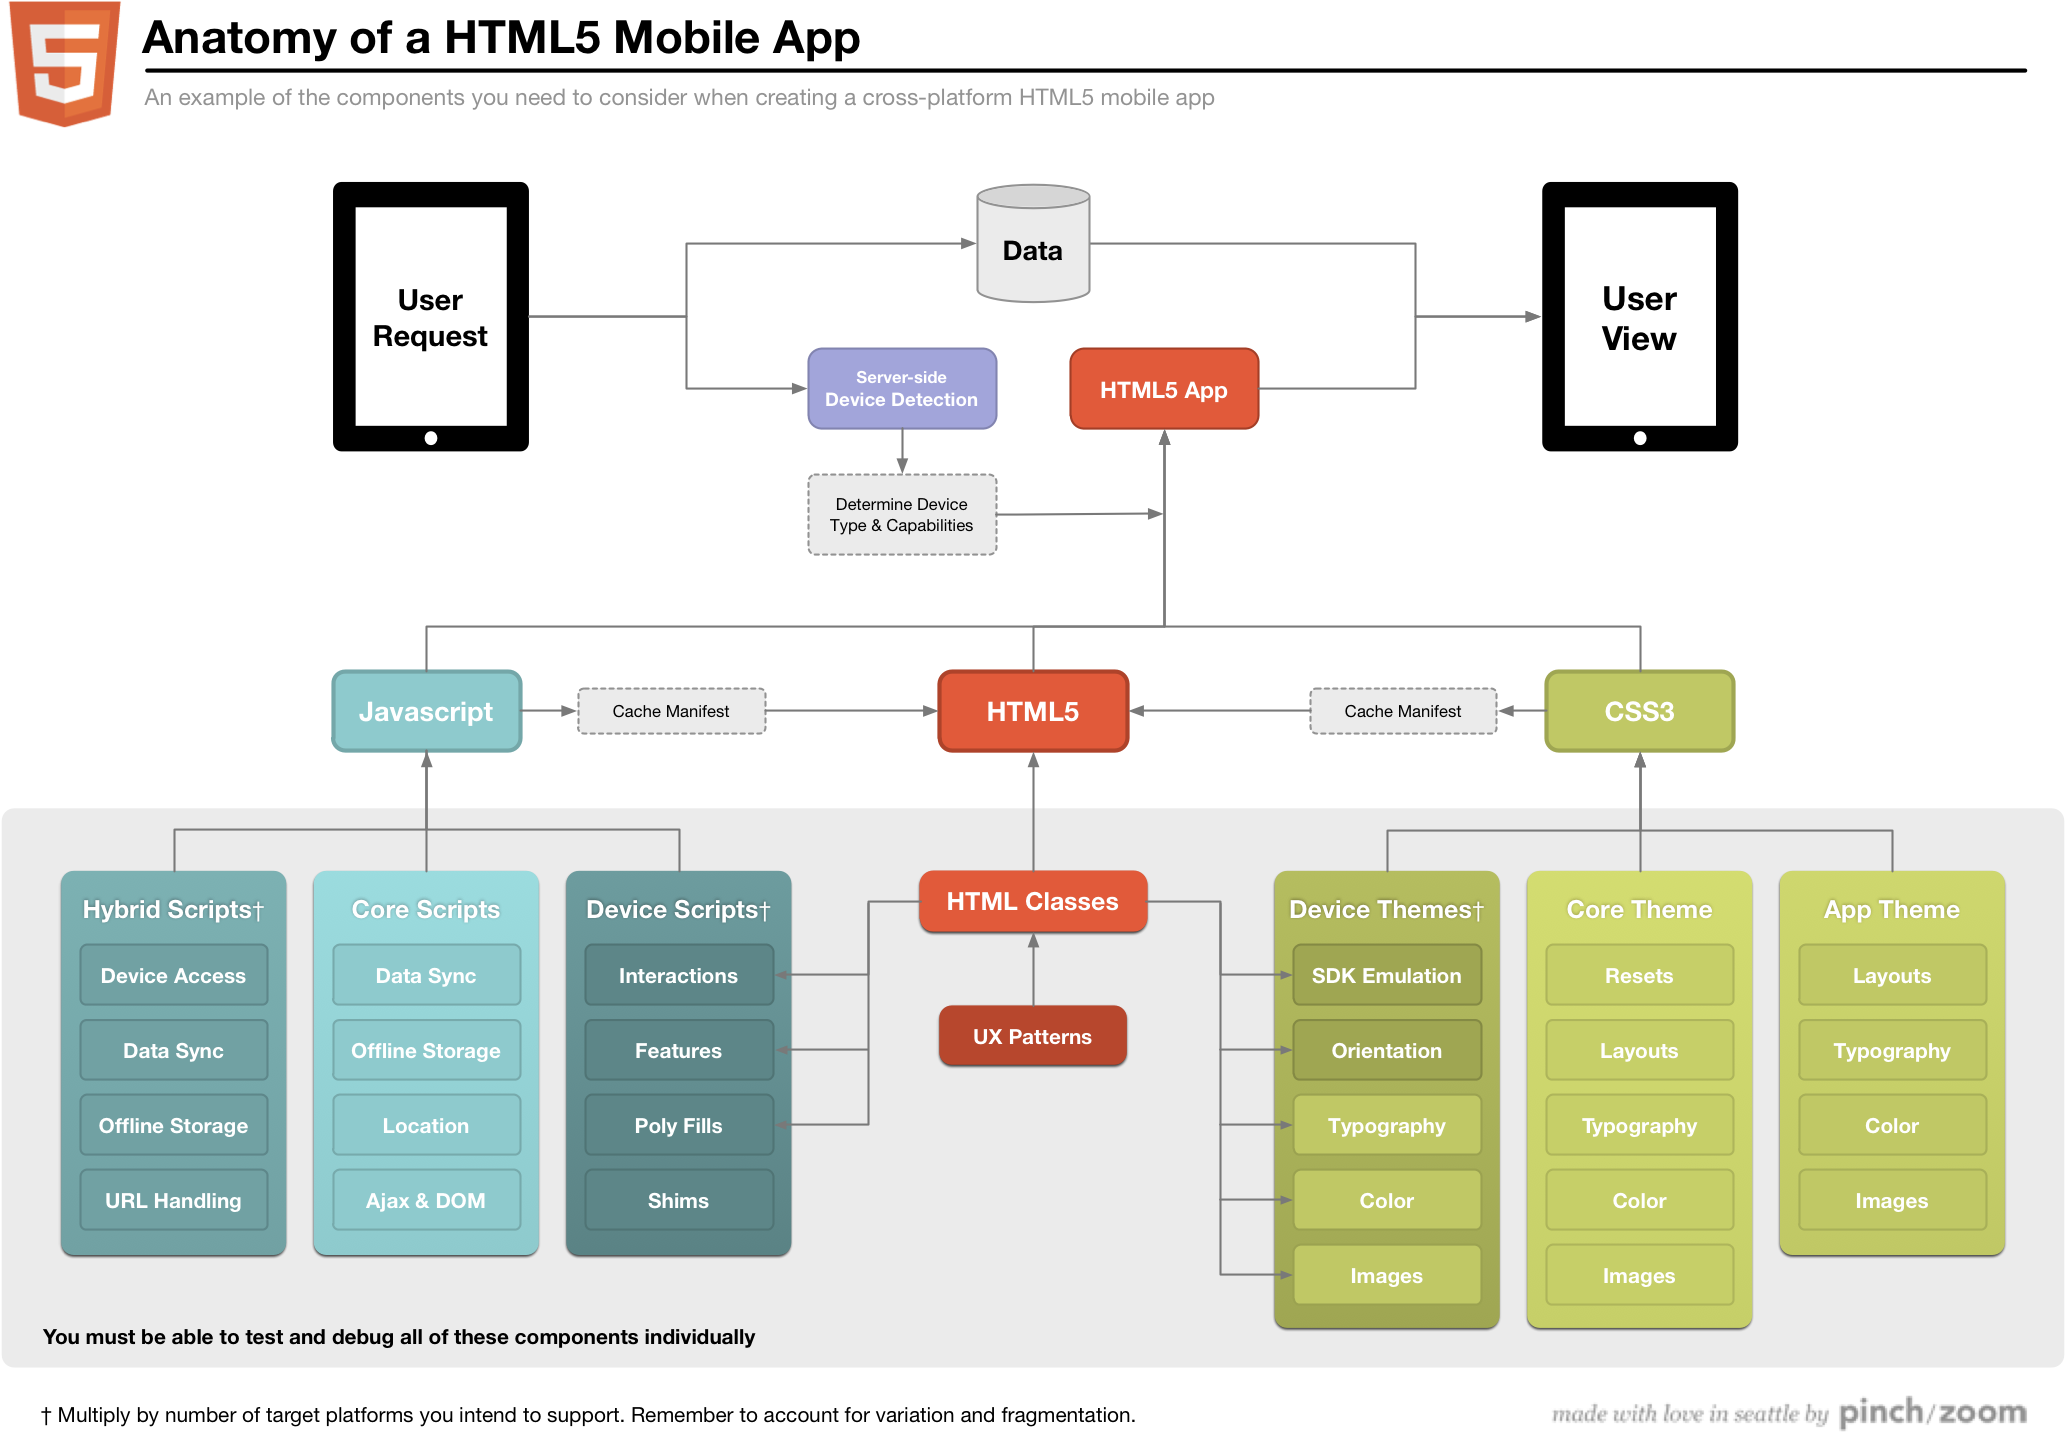
\includegraphics[width=\textwidth]{images/anatomy-of-a-html5-mobile-app.png}
  \caption{HTML5 Mobile Application Anatomy according to
    \cite{fling2011anatomy}.}
  \label{figure:anatomy-of-a-html5-mobile-app.png}
\end{figure}

In this chapter, I present tools, libraries, and techniques for
building modern web applications.

\section{Single-Page applications}
\label{section:single-page-applications}

In recent years, the movement from traditional interlinked documents
to interactive web applications has had a profound effect on the
architecture of web applications. Traditional web sites have
structured backend architectures often with a database layer, a layer
for business logic, and a layer for generating the HTML documents from
a template. The frontend usually uses \abbr{CSS} for layout and
styling and some JavaScript for enhancing forms or some interactive
components on the page.

These conventional three-tiered web applications
\cite{laine2011towards} often use an \abbr{MVC} \cite{gamma1995design}
framework for separating the data, logic, and presentation layers in
the backend. However, the latest trend in web application development
has been having only a simple \abbr{REST}
\cite{fielding2000architectural} API as a backend data layer, and
using a JavaScript MVC framework in the frontend. Thus the whole
application logic and presentation has moved to the client side, with
the backend only working as a data persistency layer.

Using modern JavaScript storage APIs (see
Section~\ref{section:datastorage}), even the data persistency and
application state layer can be in the client side, with backend only
working as an application and data delivery layer. In addition to the
client side data persistency, the storage APIs can be used to store
the user-specific application state.

Single-page applications might introduce bigger initial page load, but
after the startup, the network is only used when interacting with the
backend data API. This makes the applications faster and more
responsive, and minimizes the effects that unreliable networks have on
the application usage since separate page views do not require a new
document request.

\section{JavaScript MVC Libraries}
\label{section:js-mvc}

Due to the recent trend to move application logic from the backend to
the frontend, JavaScript code bases have grown into large applications
that need a proper modular structure. Several frameworks have been
developed to structure JavaScript applications into well-separated
modules and layers.

Many of the JavaScript application frameworks are derived from the MVC
architecture pattern adapting it to the design needs and requirements
of browser-based applications. Example frameworks include
Backbone.js\footnote{\url{http://backbonejs.org/}},
Spine\footnote{\url{http://spinejs.com/}},
ember\footnote{\url{http://emberjs.com/}},
batman.js\footnote{\url{http://batmanjs.org/}},
Knockout\footnote{\url{http://knockoutjs.com/}}, and
JavaScriptMVC\footnote{\url{http://javascriptmvc.com/}}.

One popular framework nowadays is Backbone.js, which I also chose for
the application described in
Chapter~\ref{chapter:use-case}. Backbone.js is an open source
JavaScript framework providing the essential components and structures
for building large JavaScript applications. Backbone.js provides the
following components:

\begin{itemize}
\item \textbf{Model}

  Models provide the domain-specific data layer of the
  application. They provide data manipulation, persistency, and
  serialization methods as well as an event handling mechanism for
  data changes.

\item \textbf{Collection}

  Collections are ordered sets of models. They can be used to observe
  and manipulate models as a group. They can also be used to filter
  specific models for some purposes.

\item \textbf{Router}

  Routers provide methods for routing between pages of an application
  by observing and modifying the \abbr{URL}. URLs can be mapped to
  events and actions for client-side application navigation.

\item \textbf{History}

  The History utility is used together with Routers to handle the
  application navigation to preserve the back button functionality and
  the bookmarking of certain pages in the application.

\item \textbf{Sync}

  The Sync utility provides data synchronization to the backend.

\item \textbf{View}

  Views are structures that help organizing the user interface into
  logical parts. They usually observe certain models or collections
  for changes, and update themselves independently of each other when
  the underlying data changes. They are often used together with some
  templating library, such as
  Mustache\footnote{\url{http://mustache.github.com/}} or
  Handlebars\footnote{\url{http://handlebarsjs.com/}}.

\end{itemize}

\section{Responsive Design}

Responsive design is a way to design a web page to fit to varying
sizes of screens and devices. The traditional way to design a web page
is to compromise on a certain width based on the expected desktop
screen sizes of the target audience and to lay out the elements of the
page to the chosen width.

Using Media Queries (see Section~\ref{section:css}), we can provide
tailored layouts for different screen sizes. For example, we can swap
the images to smaller ones for mobile devices or hide some elements to
make the layout cleaner on small screens. This enables us to use the
same code base to target all devices and screens.

\section{Progressive Enhancement}
\label{subsection:progressive-enhancement}

Modern web sites and web applications are accessed with a huge variety
of devices and form-factors with varying capabilities, and supporting
all the possible browsers your users might have becomes a huge burden
on developers. New standards support and \abbr{APIs} in latest
browsers seem tempting and valuable, but having to support also
less-capable browsers prevent developers from using a single solution
for all browsers.

The goal of progressive enhancement is to provide universal access to
a web site or an application no matter what capabilities the browser
or the user has. Parker et al. define the three key principles of
progressive enhancement \cite{parker2010designing}:

\begin{itemize}
\item Start with clear content and well-structured markup.
\item Maintain strict separation of layout and presentation.
\item Unobtrusively layer in advanced behavior and styling, with
  careful consideration of accessibility implications.
\end{itemize}

Often the design is started ``mobile first'' meaning that the simplest
and the most universal bottom layer of the application is designed for
the least-capable browsers with very little screen estate. This forces
the design to be simple and semantic, and filters out any extra markup
that is not needed for the semantic presentation of the content and
functionality. In addition, by designing first to browsers that might
not even have \abbr{CSS} support forces a clear separation of layout
and content as well as makes the clean markup easier to style and
enhance \cite{parker2010designing}.

Using feature detection (see Section~\ref{section:feature-detection}),
more layers are added on top of the clean markup. The objective is to
use unobtrusive JavaScript to enhance the markup to avoid breaking
parts of the page or the whole site with careless scripting. By using
feature detection, we ensure that we take the most out of the latest
browsers by using their full capabilities, and at the same time,
keeping the application accessible and functional in less-capable
browsers. This also makes the applications future-proof when browsers
are updated and new APIs and features are implemented in
them. \cite{parker2010designing}

\section{User Interface Libraries}

User Interface libraries help in developing mobile web applications
fast by providing finished and tested widgets and user interface
components that can be combined and configured easily. I present some
popular frameworks in the following sections.

\subsection{jQuery Mobile}

jQuery Mobile\footnote{\url{http://jquerymobile.com/}} is a client
side framework optimized for touch devices. The user interface is
based on HTML5 and the jQuery JavaScript
framework\footnote{\url{http://jquery.com/}}. The aim of the project
is to provide a progressively enhanced web framework for as many
devices as possible. Figure~\ref{figure:jquerymobile.png} shows
example components in the framework.

\begin{figure}[h!]
  \begin{center}
    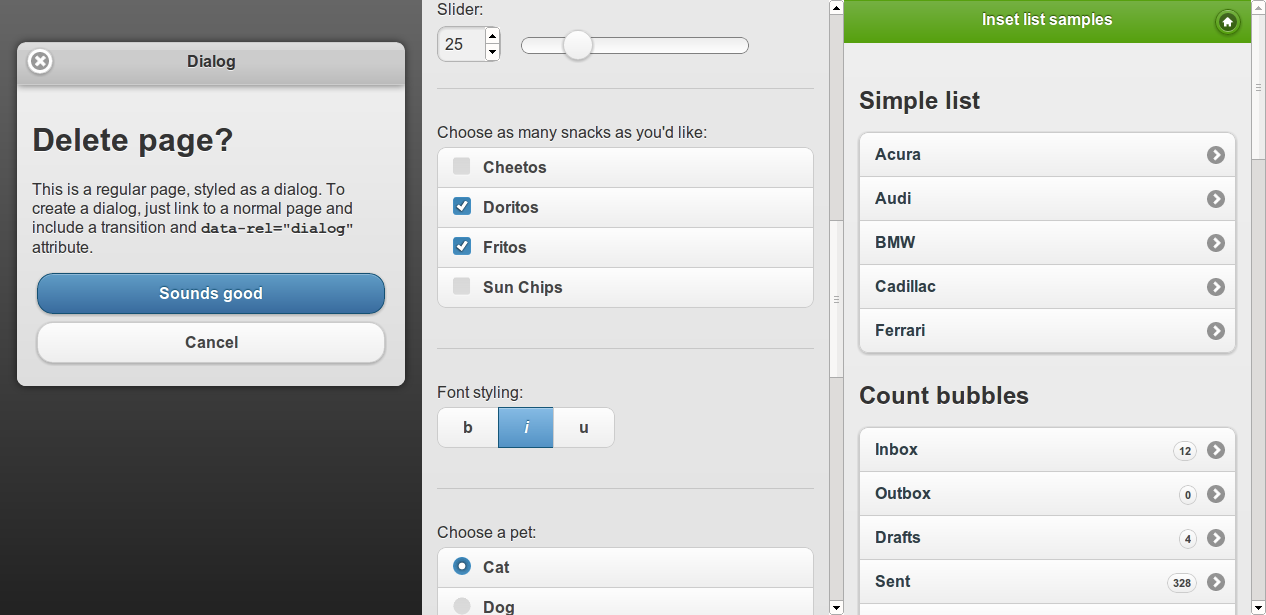
\includegraphics[width=\textwidth]{images/jquerymobile.png}
    \caption{jQuery Mobile user interface
      components. \url{http://jquerymobile.com/demos/1.0.1/}}
    \label{figure:jquerymobile.png}
  \end{center}
\end{figure}

jQuery Mobile is an open source project sponsored by large mobile and
media companies. The user interface is fully theamable and there are
several third-party extensions and widgets to the framework.

\subsection{jQTouch}

jQTouch\footnote{\url{http://jqtouch.com/}} is a lightweight open
source library for high-end smartphones and tablet devices. It only
supports the WebKit browser
engine \footnote{\url{http://www.webkit.org/}} used in iOS, Android,
Blackberry, and WebOS devices. It provides customizable themes and
user interface components, as well as helpers for handling touch
input. Figure~\ref{figure:jqtouch.png} shows example components of the
library.

\begin{figure}[h!]
  \begin{center}
    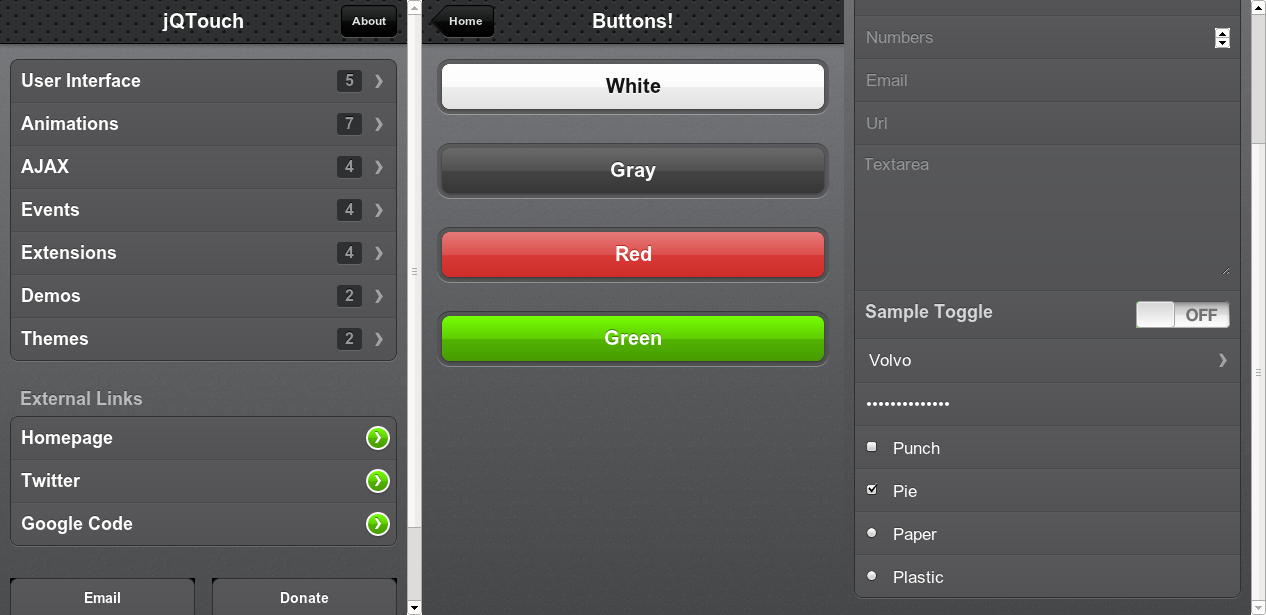
\includegraphics[width=\textwidth]{images/jqtouch.png}
    \caption{jQTouch user
      interface. \url{http://jqtouch.com/preview/demos/main/}}
    \label{figure:jqtouch.png}
  \end{center}
\end{figure}

\subsection{Sencha Touch}

Sencha Touch\footnote{\url{http://www.sencha.com/products/touch}} is
an open source HTML5 mobile web application framework for iPhone,
Android, and Blackberry devices. The framework is fully theamable and
comes with a large set of user interface components. It also provides
helpers for touch input handling. Figure~\ref{figure:sencha.png} shows
example components of the library.

\begin{figure}[h!]
  \begin{center}
    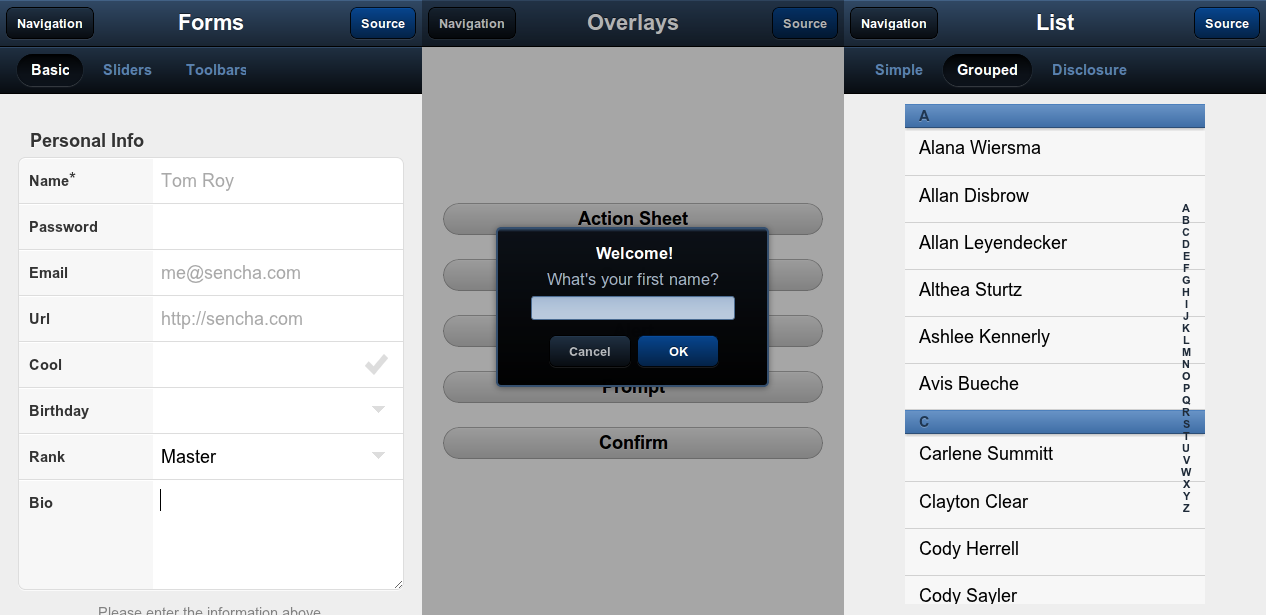
\includegraphics[width=\textwidth]{images/sencha.png}
    \caption{Sencha Touch user
      interface. \url{http://dev.sencha.com/deploy/touch/examples/kitchensink/}}
    \label{figure:sencha.png}
  \end{center}
\end{figure}

\section{Hybrid Applications}

Sometimes application stores can be a valuable marketing path, and
visibility in these stores can bring a lot of users to an
application. The stores also provide easy billing of applications
themselves, and solutions for in-app
billing. \cite{cortimiglia2011mobile}

Fortunately, modern smartphone and tablet platforms provide a user
interface component to embed a web browser view into a native
application. This web view component can be used to build parts or
even the whole application with web technologies. For example, the web
view can take the whole available screen space of the application, and
show a local HTML document together with local assets like CSS and
JavaScript files and images.

These applications that use a native web view wrapper with parts of
the application built with web technologies are called hybrid
applications. The level of native versus web technologies can vary,
and everything is possible from fully utilizing web technologies with
just a simple native wrapper to a native application with just a
simple static HTML document.

Several tools have been developed to build hybrid applications. One of
these is PhoneGap \footnote{\url{http://phonegap.com/}}, which is an
open source HTML5 application platform for building native
applications with web technologies. PhoneGap provides native wrappers
for all of the largest mobile platforms, and exposes extra JavaScript
APIs that are not accessible in normal web pages. These APIs are based
on the latest specifications, and they can be used to access device
functionality that has previously been inaccessible using JavaScript.

With tools like PhoneGap, developers can build native applications
using familiar web technologies with access to native features and
device APIs. These hybrid applications have only one code base that is
deployed for several smartphone platforms, and the applications can be
submitted to application stores.

\section{Performance Guidelines}
\label{section:performance-guidelines}

There are several web application performance best practices and
related guidelines. According to Souders \cite{souders2007high}, only
10--20\% of the end user response time is spent generating and
transferring the HTML document from the web server to the
client. Therefore, most of the optimization should be done in the
frontend for best improvement opportunities. Below I list the
performance guidelines defined by Souders \cite{souders2007high}.

\begin{itemize}

  % High Performance Web Sites

\item \textbf{Make Fewer HTTP Requests}

  According to Souders, 80--90\% of the end user response time is
  spent downloading components on a page other than the requested HTML
  page. Therefore, the simplest way to improve the response time is to
  reduce the number of HTTP requests needed to get all the required
  components.

  There are several ways to reduce the number of needed HTTP
  requests. Combining images into sprites, inlining images, or
  combining separate JavaScript and CSS files results in fewer
  components needed to download on a page.

\item \textbf{Use a Content Delivery Network}

  As web applications are deployed and become accessible worldwide,
  latency might become an issue for users far from the application's
  web servers. Geographically distributed servers allow for serving
  the application as close to the user as possible.

\item \textbf{Add an Expires Header}

  Avoiding an HTTP request altogether is the best option for reducing
  the response time when downloading the components on a page. Good
  caching strategies help browsers to know which resources are valid
  and for how long until they should be updated.

  The Expires header in HTTP tells the client how long a resource is
  valid, and especially far future Expires headers reduce the need for
  downloading and updating the components on a page after the initial
  download.

\item \textbf{Gzip Components}

  Compressing HTTP responses is an easy and effective way to reduce
  the size of the data needed to transfer across the
  network. Compression is supported widely in web browsers and the
  impact of reduced response sizes is huge. Using Gzip, the response
  size is reduced generally about 70\%.

\item \textbf{Put Stylesheets at the Top}

  Putting the CSS files to the top of the document allows the page to
  load progressively and the browser to show visual feedback to the
  user as early as possible.

\item \textbf{Put Scripts at the Bottom}

  Because scripts block parallel downloads, they should be included to
  the page after all other resources. They also block progressive
  rendering of all content below them in the HTML document, and should
  therefore be at the bottom of the document.

\item \textbf{Avoid CSS Expressions}

  CSS expressions are a way to dynamically set CSS properties in
  Internet Explorer by evaluating a JavaScript code in a
  stylesheet. However, despite the obvious upsides, the expressions
  are evaluated at such a high frequency that they negatively impact
  the performance.

\item \textbf{Make JavaScript and CSS External}

  There are performance tradeoffs between making JavaScript and CSS
  external versus inlining them in the HTML document. In the typical
  case, however, making them external enables the browser to leverage
  the HTTP caching semantics and thus reduces the needed network
  transfer.

\item \textbf{Reduce DNS Lookups}

  Apart from cached \abbr{DNS} lookups, the browser typically needs
  20--120 milliseconds to look up the \abbr{IP} address for a given
  hostname. The cache lifetime of a lookup depends on the \abbr{TTL}
  value of the DNS record and having the components of a page
  distributed across several domains might accumulate into a
  noticeable response time.

  There is also a trade-off between unique hostnames and allowed
  parallel connections and therefore these settings should be
  configured based on the application architecture and needs.

\item \textbf{Minify JavaScript}

  Because JavaScript is an interpreted language that must be sent to
  the web browser as source code, minifying the code reduces the
  required network transfer. Minifiers and obfuscators optimize the
  size of the source code by stripping extra whitespace and comments
  as well as renaming variables and function names to shorter ones
  without changing the interpreted behavior of the code.

\item \textbf{Avoid Redirects}

  Rerouting any component on a page takes time, and avoiding any kind
  of redirects improves the response times.

\item \textbf{Remove Duplicate Scripts}

  Including a resource several times serves no purpose but is actually
  quite common. Developers should make sure to include resources only
  once.

\item \textbf{Configure ETags}

  \abbr{ETags} are a mechanism in HTTP for servers and browsers to
  validate cached resources. The typical default values set by
  commonly used web servers might hurt performance, and should thus be
  configured properly to address the application architecture and
  needs.

\item \textbf{Make Ajax Cacheable}

  Highly dynamic web sites have a lot of \abbr{Ajax}
  \cite{garrett2005ajax} functionality, and developers should make
  sure all the requested URLs for data fetching follow the performance
  best practices such as having proper caching in place.

\end{itemize}

In addition to the performance rules \cite{souders2007high}, Souders
also specifies additional techniques to improve performance
\cite{souders2009even}:

\begin{itemize}

  % Even Faster Web Sites

\item \textbf{Splitting the Initial Payload}

  Nowadays, web sites include a lot of resources and JavaScript
  functionality, but only a small part of the downloaded components
  are used in the typical use cases of the application. Splitting the
  resources into bundles that can be lazily downloaded when first
  needed reduces the initial payload needed to transfer on application
  startup.

\item \textbf{Loading Scripts Without Blocking}

  Most browsers block the downloads of other resources when scripts
  are being downloaded and executed. There are several ways to
  circumvent this behavior to allow browsers to download scripts in
  parallel with other resources as well as with other script files.

\item \textbf{Coupling Asynchronous Scripts}

  Related to the previous item, when using parallel downloads with
  scripts that are dependent on each other, race conditions might
  occur due to the varying order of download and execution. Therefore,
  asynchronous scripts dependent on each other should be coupled to
  preserve the correct order of execution.

\item \textbf{Positioning Inline Scripts}

  Inline scripts do not introduce an HTTP request, but they can still
  block parallel downloads of other resources and they might affect
  also the progressive rendering of the page. With the correct
  positioning of the scripts, these problems can be handled properly.

\item \textbf{Writing Efficient JavaScript}

  After networking, the obvious place to optimize the runtime speed of
  a web application is the JavaScript code.

  Because the whole user interface and the JavaScript code run in the
  same browser thread, there can be only one thing happening at a
  time. Long running functions block the user interface from updating
  and can result in bad user experience.

  Splitting the running code into properly sized chunks, appropriately
  leveraging the asynchronous patterns of JavaScript in the
  application architecture, understanding the details and slow parts
  of the DOM API, and using several JavaScript programming best
  practices can result in big improvements in the perceived
  application performance. \cite{zakas2010high}

\item \textbf{Scaling with Comet}

  For real-time data-driven applications, there are various
  optimization techniques related to optimizing the constant data
  transfer between the server and the client. The collection of there
  various technologies is unofficially called Comet.

\item \textbf{Going Beyond Gzipping}

  Although Gzipping is widely supported in web browsers, there are
  cases when it is not supported or when the support is not
  indicated. Stripping extra content such as unneeded whitespace and
  comments reduces the payload size for uncompressed responses. There
  are also ways to detect Gzip support if the client does not directly
  indicate that.

\item \textbf{Optimizing Images}

  Images typically tend to account for a large portion of the page
  weight, and since the page weight is highly correlated to the
  response time, images are a natural target for optimization. There
  are several ways to optimize images either with lossy or lossless
  conversions.

\item \textbf{Sharding Dominant Domains}

  By tuning the amount of unique hostnames used for serving all the
  resources of an application, parallel downloads can be better
  leveraged. Also, by using HTTP 1.0 with proper Keep-Alive headers or
  HTTP 1.1 with proper persistent connections the parallel downloads
  can be tuned for better performance.

\item \textbf{Flushing the Document Early}

  Some web application frameworks allow flushing parts of the document
  to the user before the whole document is generated. This enables
  progressive rendering and gives faster feedback to the user and thus
  improves the perceived performance.

\item \textbf{Using Iframes Sparingly}

  Iframes enable developers to embed a separate HTML document inside
  another document. They are useful in sandboxing external documents
  in the same view, but the \texttt{iframe} element is the most
  expensive DOM element related to the page performance.

\item \textbf{Simplifying CSS Selectors}

  There are several ways to choose elements in CSS stylesheets to
  apply the defined properties to. Some selectors are faster than
  others and some have terrible performance.

\end{itemize}
